\documentclass[11pt, english]{article}
\usepackage{graphicx}
\usepackage[left=2cm,right=2cm,top=2cm]{geometry}
\usepackage[colorlinks=true, linkcolor=blue]{hyperref}
\usepackage[english]{babel}
\selectlanguage{english}
\usepackage[utf8]{inputenc}
\usepackage{dirtree}
\usepackage[svgnames]{xcolor}
\usepackage{caption}
\usepackage{subcaption}
\usepackage{afterpage}
\pagestyle{plain}
\usepackage{here}
\usepackage{amsmath}
\usepackage{amsfonts}
\usepackage{float}
\usepackage{epsfig}
\usepackage{epsf}
\usepackage{scrextend}
\usepackage{enumitem} % control spacing of enum
%% SCHEMA BLOC
\usepackage{tikz}
\usetikzlibrary{shapes,arrows,positioning,calc}
\tikzset{
block/.style = {draw, fill=white, rectangle, minimum height=3em, minimum width=3em},
tmp/.style  = {coordinate},
sum/.style= {draw, fill=white, circle, node distance=1cm},
input/.style = {coordinate},
output/.style= {coordinate},
pinstyle/.style = {pin edge={to-,thin,black}
}
}


\textheight=21cm
\textwidth=17cm
%\topmargin=-1cm
\oddsidemargin=0cm
\parindent=0mm
\pagestyle{plain}

\usepackage{color}
\usepackage{ragged2e}
\usepackage{listings}

\gdef\@date{ Course 2018/ 2019}


%New colors defined below
\definecolor{codegreen}{rgb}{0,0.6,0}
\definecolor{codegray}{rgb}{0.5,0.5,0.5}
\definecolor{codepurple}{rgb}{0.58,0,0.82}
\definecolor{backcolour}{rgb}{0.95,0.95,0.92}

%Code listing style named "mystyle"
\lstdefinestyle{mystyle}{
  backgroundcolor=\color{backcolour},   commentstyle=\color{codegreen},
  keywordstyle=\color{magenta},
  numberstyle=\tiny\color{codegray},
  stringstyle=\color{codepurple},
  basicstyle=\footnotesize,
  breakatwhitespace=false,
  breaklines=true,
  captionpos=b,
  keepspaces=true,
  numbers=left,
  numbersep=5pt,
  showspaces=false,
  showstringspaces=false,
  showtabs=false,
  tabsize=2
}

%"mystyle" code listing set
\lstset{style=mystyle}



\begin{document}

\begin{titlepage}

\begin{center}
\vspace*{2in}
\vspace*{-1in}
\begin{figure}[htb]
\begin{center}
\includegraphics[width=8cm]{img/logo_ircam.png}
\end{center}
\end{figure}

IRCAM ATIAM - \@date\\

\vspace*{0.4in}
\begin{large}
LATENT SPACE ORGANISATION OF \\
SOUNDS WITH VARIATIONAL AUTOENCODERS\\
\end{large}

\vspace*{0.3in}
\begin{large}
Caillon, Antoine \\
Dakeyo, Jean-Baptiste \\
Fouilleul, Martin \\
Geoffroy, Thibault \\
\end{large}
\vspace*{0.3in}
\rule{80mm}{0.1mm}\\
\vspace*{0.1in}
\begin{large}
Supervised by: \\
Adrien Bitton \\
\& \\
Philippe Esling \\
\end{large}
\vspace*{0.3in}
\includegraphics[width=2cm]{img/atiam.png}
\end{center}
\end{titlepage}

\newcommand{\CC}{C\nolinebreak\hspace{-.05em}\raisebox{.4ex}{\tiny\bf +}\nolinebreak\hspace{-.10em}\raisebox{.4ex}{\tiny\bf +}}
\def\CC{{C\nolinebreak[4]\hspace{-.05em}\raisebox{.4ex}{\tiny\bf ++}}}

\tableofcontents
\newpage
\section*{Introduction}

This project aimed to observe the organisation of sounds encoded in the latent space of an auto-encoder, and to obtain a preferably \textit{real-time} generative model, based on a chosen training set and a carefully designed architecture.

In this paper, we will firstly detail the preliminary work we performed prior to the designing of our architecture, then we will go on and present \textit{Ukulelatent}, the first system we designed, and finally we will present an idea for a second system, to be implemented in the future.
All the code relevant to this project is available at this address: \href{https://github.com/nebularnoise/serge}{https://github.com/nebularnoise/serge}.

\section{Preliminary work}
\subsection{Auto-encoders, Variational auto-encoders, Regularization}

An auto-encoder is a type of artificial neural network where two applications named \textit{encoder} ($\mathcal Q$) and \textit{decoder} ($\mathcal G$) are defined as: $\mathcal Q: x \longrightarrow z \in \mathbb Z$, and $\mathcal G: z \in \mathbb Z \longrightarrow r$, with $\mathbb Z$ the latent space and $r$ the reconstruction of $x$, with hopefully $r \approx x$.

\begin{figure}[!h]
    \centering
    \includegraphics[width=.7\linewidth]{img/architecture_ae.png}
    \caption{Architecture of a AE applied to the MNIST dataset (\textit{towarddatascience.com})}
    \label{fig:schema_AE}
\end{figure}

Classical auto-encoders can be very powerful in terms of reconstruction, at the expense of having a meaningful latent space. Since we are interested in building a generative model, the first step to consider is to incorporate a regularisation step during the training phase.\newline

Let $\mathcal Q: x \longrightarrow (\mu, \sigma)$ be an application encoding an input $x$ into a pair of latent variables $(\mu, \sigma)$, called a \textit{stochastic} encoder. We can then sample the distribution $\mathcal N(\mu, \sigma)$ to get our latent variable $h$. The whole point of having a stochastic encoder is to force it to \textit{generalize} by regularizing the latent space. Classical VAEs define a loss based on the KL divergence between the encoder's output and a prior distribution\footnote{\label{foot:appendix}More detail in appendix \ref{sec:appendix}}. The encoder's output is then forced to look like this prior; the choice of a good prior is thus extremely important to have satisfying results.\newline

In our case, we use a slightly different way to regularize our latent space. Instead of forcing $(\mu, \sigma)$ to correspond to our prior, we consider the whole encoder's output $\mathcal Q(\underline x)$ given a batch of inputs $\underline x$, and compute the discrepancy between this output and a prior, via the \textit{Maximum Mean Discrepancy} method \footref{foot:appendix}. This method requires us to choose between different kernels in order to estimate this discrepancy (RBF, IMQ).

\subsection{Divergence Benchmark}
The aim of this part is to compare the efficiency of different divergence functions, namely:
\begin{enumerate}[noitemsep]
    \item Kullback - Leibler Divergence (KLD)
    \item Maximum Mean Discrepancy for a Radial Basis Function Kernel (MMD$_{\text{(RBF)}}$)
    \item Maximum Mean Discrepency for a Inverse Multi-Quadratic Kernel (MMD$_{\text{(IMQ)}}$)\newline
\end{enumerate}

\vspace{-0.5cm}
Each colored line displayed on Figure \ref{fig:bench} gives the corresponding divergence between our $\mathcal N(0,1)$ prior and a set of points sampled from a normal distribution, which mean is between $[0,10]$ and is defined by the color of the curve, depending on the variance $\sigma^2$.

\begin{figure}[H]
   \begin{minipage}[t]{0.05\linewidth}
      \includegraphics[scale=0.55]{img/MMD_RBF_benchmark.png}
   \end{minipage} \hfill
   \begin{minipage}[t]{0.05\linewidth}
      \includegraphics[scale=0.55]{img/MMD_IMQ_benchmark.png}
   \end{minipage} \hfill
   \begin{minipage}[t]{.35\linewidth}
      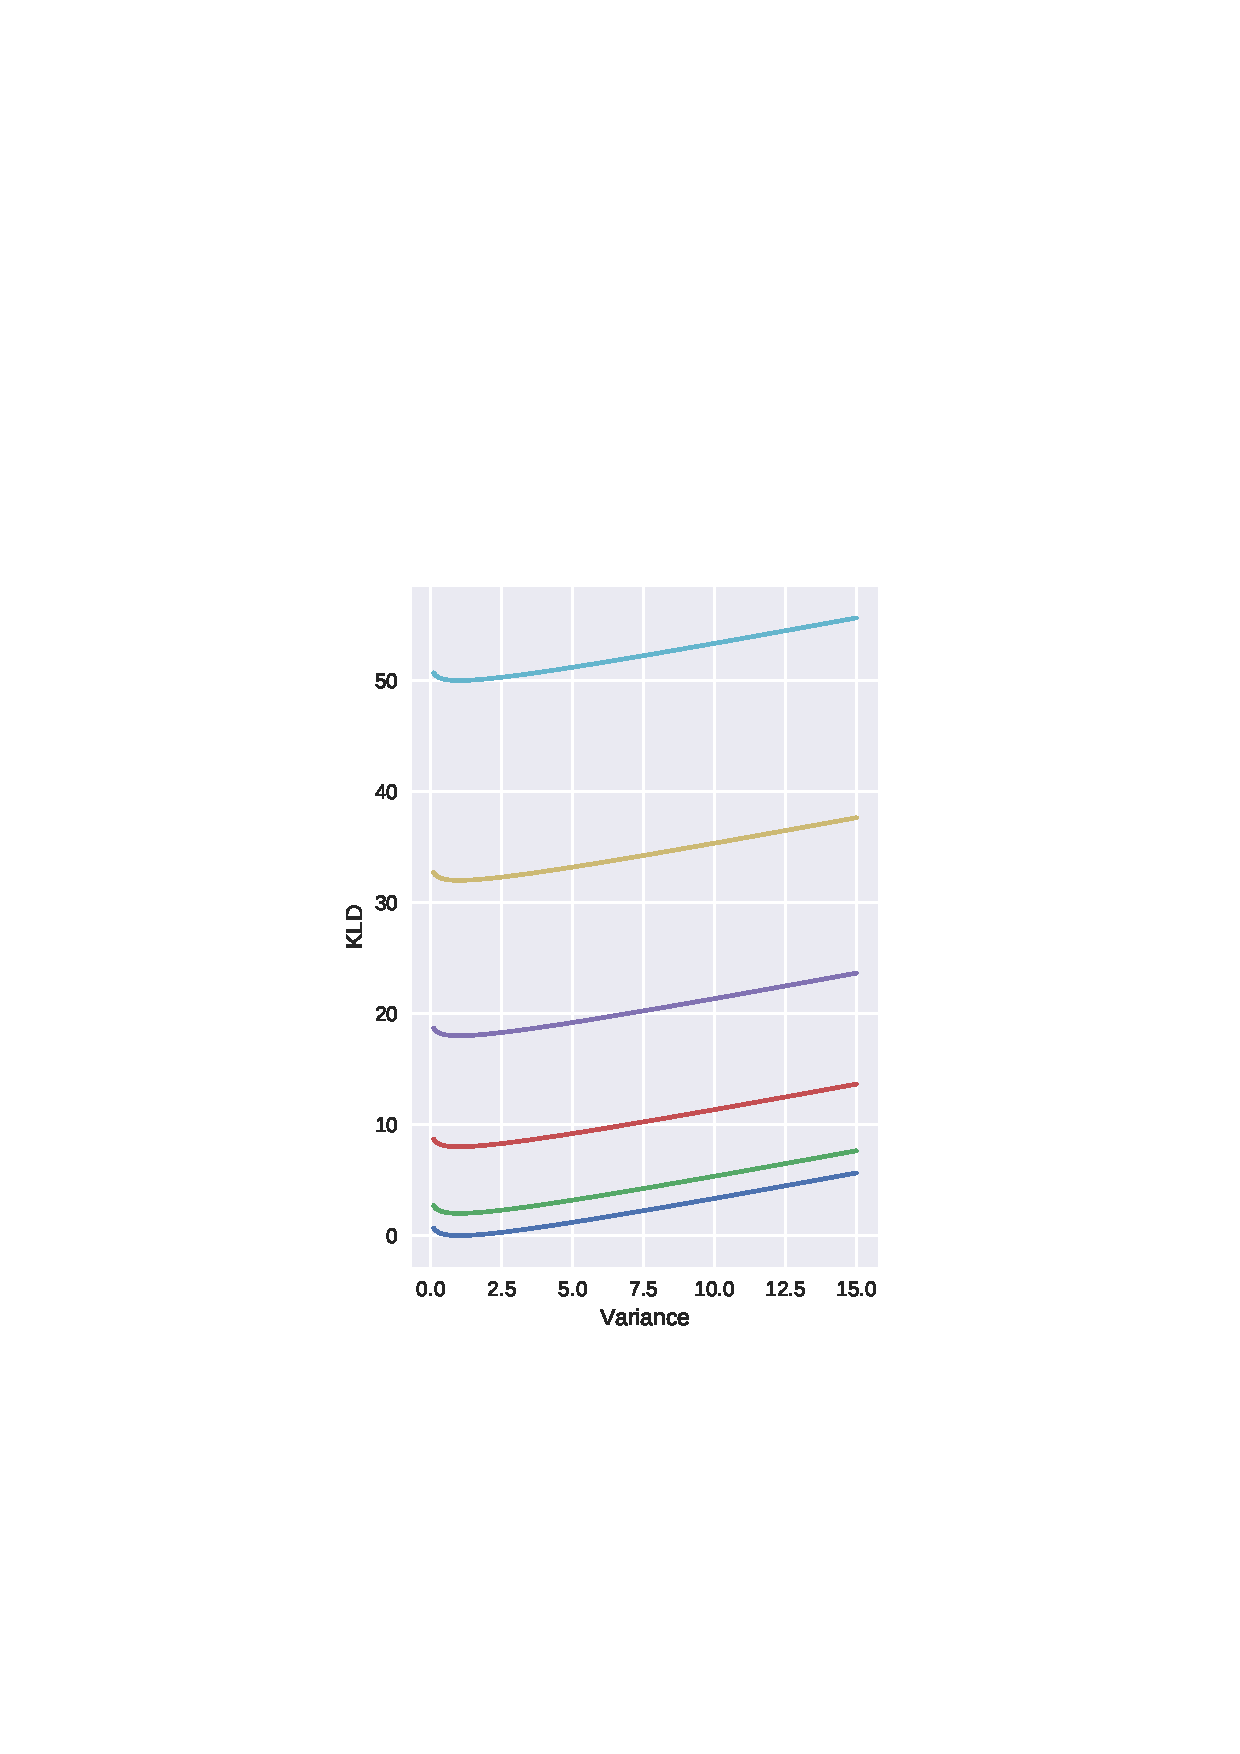
\includegraphics[scale=0.55]{img/KLD_benchmark.png}
   \end{minipage}
    \caption{Benchmark of MMD$_{\text{(IMQ)}}$, MMD$_{\text{(RBF)}}$ and KL for a standard normal prior}
    \label{fig:bench}
\end{figure}


All those divergences reach a global minimum for the distribution $\mathcal N(0,1)$ identical to our prior, which was expected, but still reassuring. The main differences between those three are their behaviour when the variance goes up. The KL divergence, being analytic, doesn't suffer from a high variance and is still able to "measure" how far the distribution is from the prior. For both MMD$_{\text{(RBF)}}$ and MMD$_{\text{(IMQ)}}$, when the mean is not 0, they decrease as the variance increase, which is not what we would have liked them to do.\newline

In practice however, the MMD$_{\text{(RBF)}}$ outperforms the KL divergence in terms of organization of the latent space. While the KL divergence tends to force the encoder to produce $\mathcal N(0,1)$ samples, the MMD$_{\text{(RBF)}}$ allows it to yield any value it wants, \textit{as long as} the continuous mixture of latent variables looks like the prior.

\subsection{Toward a MNIST VAE}

In order to get used to the AE, VAE and WAE, we played with the \textbf{MNIST} dataset, which is made of 60000 28x28 pixels handwritten digits. We first implemented a non-regularized auto-encoder and trained it with an Adam optimizer on this dataset. The encoding / decoding pass of a sample from the train set produced good reconstructions, but a small variation in latent space coordinates produces disastrous results.

\begin{figure}[h!]
    \centering
    \scalebox{0.8}{
    \begin{subfigure}[t]{.32\linewidth}
    \centering \includegraphics[width=\linewidth]{img/AE_5.png}
    \caption{Sample from the train set}
    \end{subfigure}
    ~
    \begin{subfigure}[t]{.32\linewidth}
    \centering \includegraphics[width=\linewidth]{img/AE_5_rec.png}
    \caption{Reconstruction}
    \end{subfigure}
    ~
    \begin{subfigure}[t]{.32\linewidth}
    \centering \includegraphics[width=\linewidth]{img/alien.png}
    \caption{Reconstruction with a small variation of the latent point}
    \end{subfigure}
    }
    \caption{Reconstruction on a non regularized auto-encoder}
\end{figure}

We then implemented both a variational auto-encoder(VAE) and Wasserstein auto-encoder(WAE), which yielded much better latent space organization (see Figure \ref{fig:latentspaceorg}).
While the VAE's reconstructions were much blurrier than the AE's, the WAE's latent space had a good structure, and still produced satisfying results.

\begin{figure}[h!]
\centerline{
\scalebox{1}{
    \begin{subfigure}[t]{.35\linewidth}
    \centering \includegraphics[width=\linewidth]{img/AE_Z.png}
    \caption{AE latent space}
    \end{subfigure}
    ~
    \begin{subfigure}[t]{.35\linewidth}
    \centering \includegraphics[width=\linewidth]{img/VAE_Z.png}
    \caption{VAE latent space}
    \end{subfigure}
    ~
    \begin{subfigure}[t]{.35\linewidth}
    \centering \includegraphics[width=\linewidth]{img/WAE_Z.png}
    \caption{WAE latent space}
    \end{subfigure}
    }}
    \caption{2D latent space structural differences for an AE, VAE and WAE trained on the same MNIST dataset}\label{fig:latentspaceorg}

\end{figure}

\newpage

\section{Ukulelatent: a latent ukulele sampler}

In this project we use regularized auto-encoders in order to reconstruct audio spectrograms from a latent space. Given a spectrogram $S$, we are learning two applications $\mathcal Q$ and $\mathcal G$ such as

\begin{align}
S \approx \mathcal G(\mathcal(Q(S))).
\label{S_expression}
\end{align}

The final aim is to study how the latent space is organized, hence we need a way to actually explore and \textit{hear} this space. We decided to achieve this by embedding a pre-trained \textbf{PyTorch} model inside a \textbf{PureData} external, connected to a MIDI controller.\\

This presents some challenges: we need to make our sampler \textit{real-time}, find a way to get audio from mel-spectrograms, and design a way to \textit{see} and \textit{control} our position inside the latent space intuitively.

\subsection{Dataset}

In order to get audio files to work on, we recorded about $\approx 500$ plucked strings sounds from two instruments: a \textit{motu}\footnote{A traditional instrument from the Oleron Island, akin to a small ukulele} and a classical guitar. Every sound is normalized and cropped to 34560 samples. The only two things left to compute are the \textbf{mel-spectrogram} and an estimation of the fundamental frequency of each audio files. Each mel-spectrogram's amplitude is brought between -1 and 1, log scale.

\subsection{Model}

We define $\mathcal Q$ and $\mathcal G$ as encoder and decoder respectively. Both are using several convolutive and fully-connected layers, as long as a some regularization applied to the latent space.

\subsubsection*{Architecture}

The following architecture is implemented using the \texttt{\textbf{PyTorch}} framework.

\begin{figure}[!h]
    \centering
    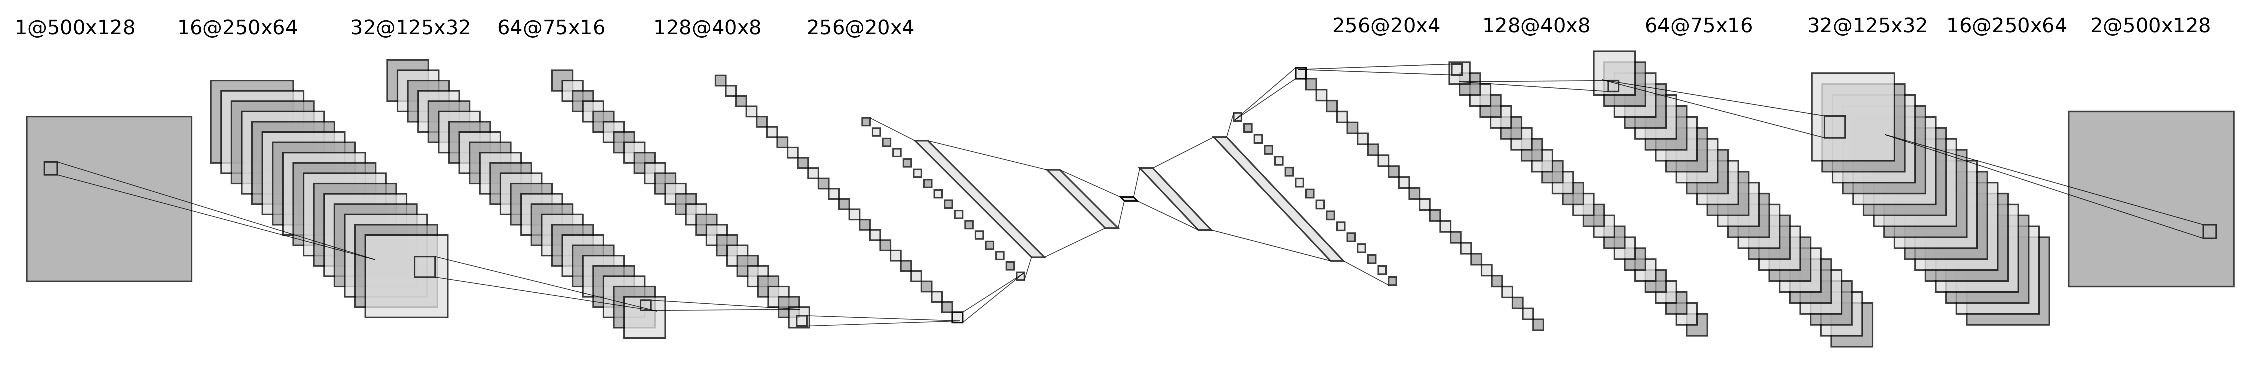
\includegraphics[width=\linewidth]{img/archi.eps}
    \caption{Architecture of the WAE used for the Ukulelatent}
    \label{fig:archi}
\end{figure}

This architecture was subject to many modifications during the course of this project. The one presented in Figure \ref{fig:archi} gave satisfying results reconstruction-wise. Both encoders and decoders are stochastic (they both yield a mean and a variance from which we can sample a value), and a regularization is applied to the latent space (see \textbf{Losses}).\\

At first we used deconvolutive layers in the decoder, to invert the convolutive layers of the encoder. We managed to make some reconstructions, but had problems with the well-known checkerboard effect, so we replaced them with upsample - convolutive layers as described in \cite{odena2016deconvolution}, resulting in smoother results (see figure \ref{fig:comparison_sample_reconstruction}).

\begin{figure}
    \centering
    \includegraphics[width=\linewidth]{img/compa_finale_specto.png}
    \caption{Comparison between a sample from the test set and its reconstruction from the WAE}
    \label{fig:comparison_sample_reconstruction}
\end{figure}

\subsubsection*{Losses}

We define the following WAE objective in equation \eqref{WAE_objective} :
\begin{align}
\mathcal L_{\text{WAE}}(x, \hat x, z) = \text{MSE}(x,\hat x) + \alpha . \text{MMD}_\text{RBF}(z),
\label{WAE_objective}
\end{align}

where $x, \hat x$ are the original and reconstructed mel-spectograms, $z = \mathcal Q(x)$, MSE the mean square error function, and $\text{MMD}_\text{RBF}$ an estimation of the maximum mean discrepancy between $z$ and a normal distribution using a standard normal kernel (\cite{ref_MMD_1}, \cite{ref_MMD_2}). We then train our model using an Adam optimizer, with an initial learning rate of $10^{-5}$ which we divide by two every $100$ epoch.

\subsubsection*{Signal reconstruction}
We first tried to use an Multi-Scale Convolutional Neural Networks (MCNN) to reconstruct the signal from the magnitude spectrogram produced by our model. After having acknowledged the fact that we had not enough training data to produce good reconstruction, especially on data outside its train set, we settled for the classical Griffin-Lim algorithm\cite{griffin_lim}.

\subsubsection*{Supervising}

While the latent space may be well organized, it is still unclear how to properly explore it. In order to finally get a sampler that we can play, we need to make the model map the audio samples to a certain midi note number. We first implemented a function estimating the fundamental frequency $f_0$ of a signal, following those steps:
\newline
\begin {enumerate}[noitemsep]
    \item Compute the biased auto-correlation estimator $R_{xx}$ of the input signal $x$
    \item Define a frequency range $[f_{\text{min}}, f_{\text{max}}]$ in which $f_0$ is included
    \item Compute the corresponding period range $[\tau_{\text{min}} = f_e / f_{\text{max}}, \tau_{\text{max}} = f_e / f_{\text{min}}]$
    \item Compute $\tau_0 = \text{argmax}(R_{xx}[\tau_{\text{min}}:\tau_{\text{max}}]) + \tau_{\text{min}}$
    \item Yield $f_0 = f_e / \tau_0$.
\end{enumerate}

This fundamental frequency method is quite cheap to compute and robust in term of identification, thus it is added to the audio dataset pre-processing pass.\newline

Next, we need to tell the model what is the fundamental frequency of the audio sample, which we tried to do in many different ways.

At first we simply mapped the frequency to an extra dimension on both the encoder and decoder, hoping the system would see that there was a correlation between a vertical shift in the mel spectrogram and the given parameter. It failed by bypassing completely our parameter.

We then tried to manually shift the input mel-spectrogram according to its estimated fundamental frequency. The encoder would therefore only ever encode sounds of the exact same fundamental frequency. On the decoder side, the system is expected to reconstruct the unshifted spectrogram by using our MIDI-note parameter. This was a failure too, as the model would just fail to reconstruct the spectrograms.\newline

Finally, we tried to pass $f_0$ as two one-hot vectors, one of size 7 (giving the octave number), and the other of size 12 (giving the semitone number), and it worked! The model was learning to map data accordingly to those two vectors, thus giving us the ability to choose the spectrogram's pitch we wanted to reconstruct.\newline

What is now interesting is to guess the purpose of the latent space's other dimensions given by the encoder, now that the pitch related information is manually encoded into two one-hots. We fixed the encoder's output dimension to 4, as we could explore it with two XY pads. By playing around with a midi keyboard, we estimated that mainly three hyper parameters are encoded in this 4-dimensional space:

\begin{itemize}[noitemsep]
    \item Amount of low frequency in the spectrum
    \item Damping
    \item Metallic-ish sounding instrument.
\end{itemize}

This intuitively sounds like an accurate way to organize the dataset, as those are parts of the main differences between a motu and a guitar. Maybe a 4-dimensional space is overscaled for this dataset, and should be upscaled for more complex ones. Using the T-SNE algorithm, we are able to \textit{unfold} the latent space in order to visualise the inner separation between samples (see fgure \ref{fig:tsne}).

\begin{figure}
    \centering
    \centerline{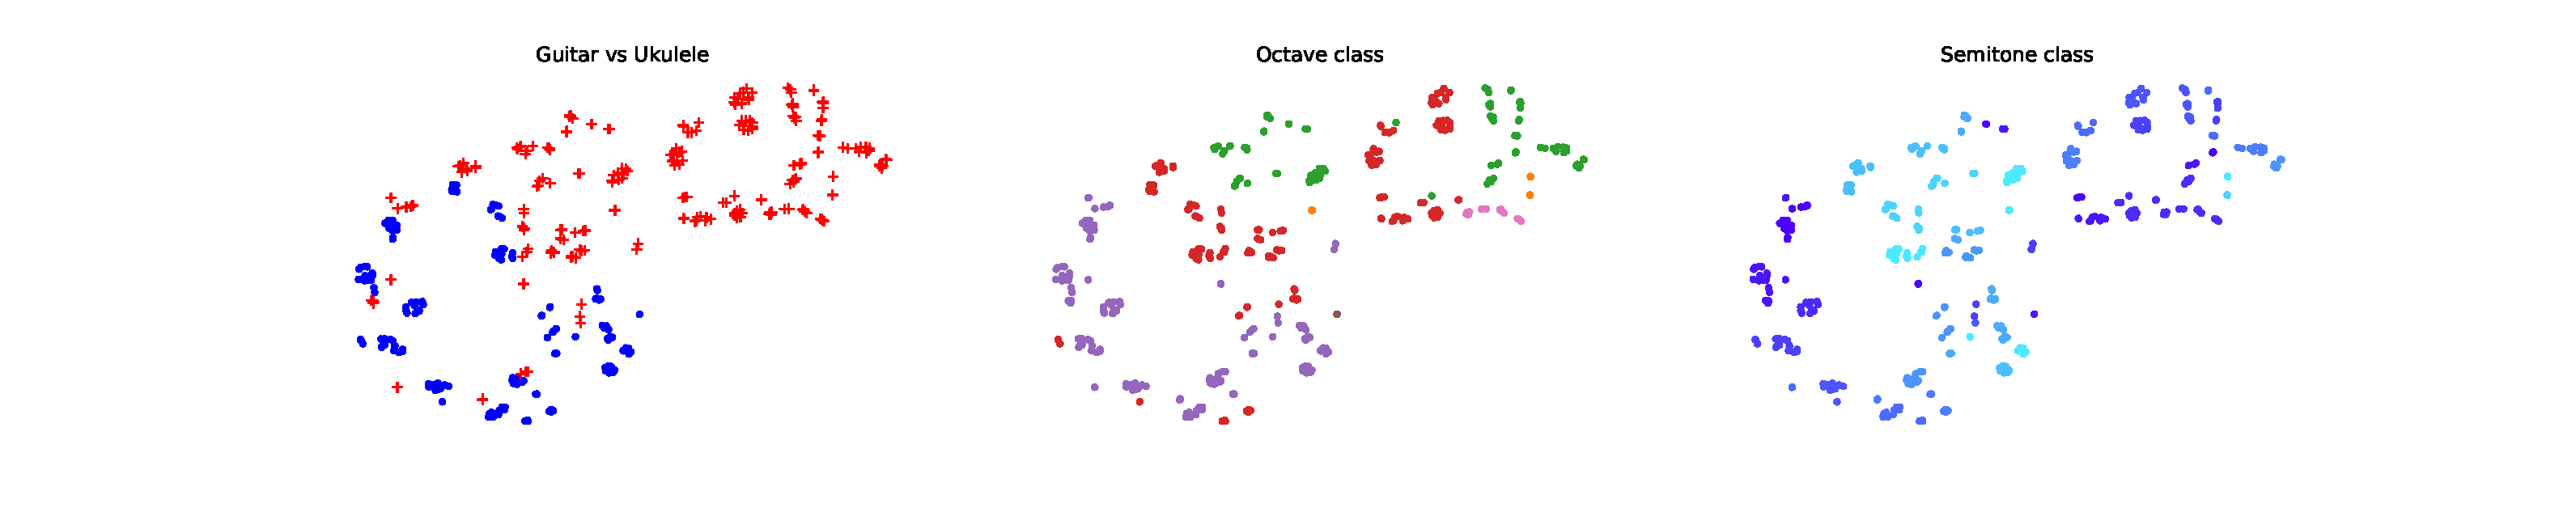
\includegraphics[width=1.3\linewidth]{img/tsne_latent_space_guitare_uku.eps}}
    \caption{2D representation of the latent space via the T-SNE algorithm}
    \label{fig:tsne}
\end{figure}

\subsection{Puredata external}

In order to allow the real-time exploration of the latent space of our pre-trained model, we embedded our model inside a \texttt{Pd} external called \texttt{vae\_sampler\~}. It can then be integrated within a patch with an adapted GUI and MIDI control.
\paragraph{}
The external has one inlet that can receive two messages :
\begin{itemize}
\item When receiving a \texttt{load} message with a file name as argument, the external loads the model from a file.
\item When receiving a \texttt{play} message with one int (corresponding to a MIDI note) and four floats (corresponding to coordinates in the latent space) as arguments, the external uses the loaded model to generate a spectrogram. It then reconstructs an audio signal from this spectrogram and outputs this signal from its audio outlet.
\end{itemize}

\subsubsection{Wrapping \texttt{libtorch}}

Using a \textbf{\texttt{PyTorch}} model from \textbf{\texttt{C++}} is made possible by leveraging the \textbf{\texttt{LibTorch}} API. The \textbf{\texttt{PyTorch}} model is first converted to \textbf{\texttt{TorchScript}} by tracing its \texttt{forward()} function with example data from the train-set, and serialized to a file. This file can then be loaded by a \textbf{\texttt{C++}} program linked to the \textbf{\texttt{LibTorch}} library. \newline
The \texttt{vae\_sampler\~} external is coded in plain \textbf{\texttt{C}}, whereas \textbf{\texttt{LibTorch}} exposes a \textbf{\texttt{C++11}} API. Hence in order to use it in our external, we wrote a wrapper that is responsible for loading the model, calling its \texttt{forward()} function and converting back and forth \textbf{\texttt{LibTorch}} tensor types.

\subsubsection{Real-time signal reconstruction}

The external has a number of polyphony voices each associated with a worker thread and an audio buffer. When requested to play a note with a given set of latent space coordinates, the external allocates a voice of polyphony and fires up its worker thread. This thread calls into our wrapper's functions to retrieve a spectrogram. It then proceeds to reconstruct the signal from the spectrogram and stream it to the voice's audio buffer, staying ahead of \textbf{\texttt{Pd}}'s audio callback. \newline
In order to reconstruct the signal inside the external with sufficient performance, we re-implemented the Griffin-Lim algorithm in \textbf{\texttt{C}}. Our implementation is based on the state-of-the-art \textbf{\texttt{FFTW}} library for fast discrete Fourier transforms. With compiler optimizations on, on our test machine, our implementation of the Griffin-Lim algorithm took 0.7s to reconstruct a 1s sample with 100 iterations. In order to eliminate most of this latency, our reconstruction function divides the spectrogram into batches of 32 DFT slices, streams the batches into the Griffin-Lim algorithm and reconstructs the signal step-by-step. We were able to reach a real time throughput using this technique.\newline
The output buffers of each voice are then read and combined by the \texttt{perform()} routine of the external, and finally sent through the signal outlet of the external.

\subsubsection{Handling the model's latency}

The model itself took 0.8s to compute a complete spectrogram on our test machine without \textbf{\texttt{CUDA}} support. We tried to build a new model which could stream the spectrogram in small batches, but we found it was much more difficult to train, probably due to the loss of internal coherence of those small batches compared to a full spectrogram. Thus the model imposes an initial latency on the audio generation.  \newline

We then wrote a wrapper around our \textbf{\texttt{C}} Griffin-Lim implementation, and used it inside a pure \textbf{\texttt{Python}} audio engine with \textbf{\texttt{CUDA}} support (see \texttt{explore\_space.py}). On a machine with an nvidia MX130 GPU, we were able to reconstruct a full mel-spectrogram in less than 60ms. A demo video is available at \href{https://youtu.be/yjcfi6fvs3o}{https://youtu.be/yjcfi6fvs3o}. \textbf{\texttt{CUDA}} support in the \textbf{\texttt{PureData}} external is still to be improved. \vspace{1cm}

\begin{figure}[!h]
    \centering
    \includegraphics[width=.8\linewidth]{img/ukulelatent_petit.jpg}
\end{figure}


\section{Latent audio effect organisation on synth samples : FX-Coast}
One objective of this project was to explore the possibilities of latent space organization of sounds processed by effects. This would require to train the model with a dataset, augmented by DSP routines.
We decided to try and have a bigger variety of sounds in the core dataset than in the previous system.

\subsection{Dataset}
For this new exploration of latent space organisation of sounds, we first developed a new core dataset. We recorded more than 2000 synth hits made with a modular system, and a Make Noise 0-coast.

After developing the core-dataset, the idea was to augment it by processing it with DSP routines.
We needed to be able to process our dataset in batches, so the ideal solution was one-liner commands. After attempting to use CSound, we decided to use Faust, out of familiarity with its ecosystem.

\begin{figure}[h]
\center
\begin{tikzpicture}[auto, node distance=2cm,>=latex']
    \node [block] (f) {'.dsp' Faust file};
    \node [block, right of=f,,node distance=6cm] (cpp) {'.cpp' file};
    \node [block, right of=cpp,node distance=4cm] (exe) {Executable};
    \draw [->] (f) -- node[name=ulabel]{\texttt{faust2sndfile}} (cpp);
    \draw [->] (cpp) -- node[name=ulabel]{\texttt{clang++}} (exe);

    \node [block, above of=exe, xshift=1.5cm] (in) {\texttt{input.wav}};
    \node [block, below of=exe, xshift=1.5cm] (out) {\texttt{output.wav}};
    \draw [->] (in) -| (exe);
    \draw [->] (exe) |- (out);
    \end{tikzpicture}
    \caption{Principle of the dataset augmentation pipeline}
    \label{fig:sch1}
\end{figure}

We needed to keep the time response relatively short for the model to be able to process the dataset. This implied that long delays and reverb sounds were out of the question, so the effects are mainly filtering and distortion effects.

After processing the dataset, we had multiplied the size of our dataset by a factor of 72, which is to say the amount of DSP routines we developed.

\subsection{The issue of time}
The idea was to reuse the architecture of the ukulelatent network, and process the FX-Coast dataset.

However, due to the sheer size of the resulting FX-Coast Dataset ($\approx$ 120 GiB), one epoch would have likely taken several hours. Given that the deadline for the project was only less than a week away, we gave up on this endeavour.

\section*{Conclusion}

Using a WAE with multiple convolutional and fully connected layers, we were able to properly reconstruct and generate mel-spectrograms, after constraining our latent space to a normal standard prior with the $\text{MMD}_\text{RBF}$ regularisation. Supervision using one-hot vectors succeeded in shifting the spectrograms in frequency.
After wrapping the \textbf{PyTorch} model in a \textbf{PureData} external, we managed to reconstruct audio in real-time using an efficient C implementation of the Griffin-Lim algorithm, and CUDA support in the external.

The resulting sampler gave satisfying results on a plucked string dataset, which was developed for the occasion.

In an effort to diversify the dataset and explore the organisation of audio effects in the latent space, we set out to develop a new system, with a larger dataset, augmented by the use of DSP routines. While the groundwork was performed, the training had to be shut down due to a lack of time. Further work could allow for a second real-time sampler using this new DSP-augmented dataset.

\bibliographystyle{plain}
\bibliography{bibliography}

\newpage
\appendix
\section{Divergences}
\label{sec:appendix}

\subsection{Kullback-Leibler Divergence}


The Kullback–Leibler divergence (KLD) measure the difference between two probability distribution ( \cite{KL_1951}, \cite{K_1959} ).
The more two distributions are similar, the closer the KLD will be to 0, and the further the distributions are, the more the divergence increases. The KLD is defined as follows :
\begin{align}
D_{KL}(P \: || \: Q) = \sum_i P(i) \ln \left( \frac{P(i)}{Q(i)} \right) ,
\end{align}

with P and Q two probability distributions of a discrete random variable.
We can also see it like the average of the logarithmic difference between P and Q.

However, the KLD is only defined if $P(i) > 0$, $Q(i) > 0 $ for any $i$, and if P and Q both sum to 1.
A simplification in the formula is possible in the case of multivariate distributions.
Suppose that we have two multivariate normal distributions, with means
$\mu_p$ , $\mu_q$ and with (non-singular) covariance matrices $\Sigma_p$ and $\Sigma_q$.
 If the two distributions have the same dimension,
$k$, then the KLD is :

\begin{equation}
D_{\text{KL}}({\mathcal {N}}_{p}\parallel {\mathcal {N}}_{q})={\frac {1}{2}}\left(\operatorname {tr} \left(\Sigma _{q}^{-1}\Sigma _{p}\right)+(\mu _{q}-\mu _{p})^{\mathsf {T}}\Sigma _{q}^{-1}(\mu _{q}-\mu _{p})-k+\ln \left({\frac {\det \Sigma _{p}}{\det \Sigma _{q}}}\right)\right).
\end{equation}



In our case, we consider a dependence to $z$ the latent space, from P and Q. We define $p(z)$ a normal prior and $q(z)$ another normal distribution. The distribution p(z) will be later sampled to generate some data, the easiest choice would be to choose $p(z) \sim \mathcal{N}(0,1)$. It is possible to write all the latent variables mutually independent and each parametized by a distinct variational parameter \cite{rapport_stage_cyran}:

\begin{align}
    q(z) = \prod_{j-1}^{m}q_j(z_j).
\end{align}


Here, each latent space $z_j$ follows an independent variational factor, defined by $q_j(z_j)$. We have made the choice to use normal factors. Thus each dimension of the latent space will be governed by an independent normal distribution with its own mean and variance, and in the VAE this is especially $q_j(z_j) = \mathcal{N}( \mu_j (\textbf{x}), \Sigma_j(\textbf{x}))$, where the parameters depend on the input data. The KLD can be computed for our VAE like :



\begin{equation}
\begin{split}
D_{\text{KL}}\left[P \: || \: Q \right] &=   D_{\text{KL}}\left[ \mathcal{N}(0,1) \: || \:  \mathcal{N}(\mu(\textbf{x}) , \sigma(\textbf{x})) \right].\\
\end{split}
\end{equation}

If the two distributions have the same dimension, k, then the KLD between them is as follows :

\begin{equation}
\begin{split}
D_{\text{KL}}\left[ \mathcal{N}(0,1) \: || \:  \mathcal{N}(\mu(\textbf{x}) , \sigma(\textbf{x})) \right]
&= {1 \over 2} \sum_{k} \left( \Sigma_q(x_k) +\mu_q^{2}(x_k) - \ln(\Sigma_q(x_k) ) - 1 \right),
\end{split}
\end{equation}

where $\Sigma_q(x_k)$ and $\mu_q(x_k)$ are respectively the variance and the mean of the $k^{th}$ dimension of Q.
This is the formula we used to measure the KLD in our VAE.

\subsection{Maximum Mean Discrepancy}
To set the Hilbert Space, we consider a reproducing Kernel Hilbert Space $\mathcal{H}$ with kernel $k$ \cite{ref_MMD_1}. To evaluate the function $f$ depending to the kernel $k$, we define : $f(x) = \langle {k(x,.),f} \rangle $ .\\
And computing means via linearity gives :

\begin{align}
    E_{p} [f(x)] &= E_p[\langle k(x,.), f\rangle ]  \\
    &= \langle E_p[k(x,.)],f \rangle ,
\end{align}

where $Ep[f(x)]$ is the expected value of the function $f$. To define the expected value, we use the Monte-Carlo method. It consist on generate samples randomly from a probability distribution \cite{monte_carlo_method}.
It is possible to represent the optimization problem as follows :

\begin{align}
    sup_{||f|| \leq 1} E_p[f(x)] - E_q[f(y)] &= sup_{||f|| \leq 1} \langle \mu_p -\mu_q , f \rangle \\
    &= ||\mu_q - \mu_q||_\mathcal{H}.
\end{align}

And if the expression is written in terms of expected values, we get :

\begin{align}
|| \mu_p - \mu_q||^2_H  &= \langle \mu_p - \mu_q, \mu_p - \mu_q \rangle \\
&= E_{p,p}k(x,x') + E_{q,q}k(y,y') - 2E_{p,q}k(x,x') .
\label{equ_mmd}
\end{align}

The variable $E_{i,j}$ is the expected value between two distribution $i$ and $j$.
The equation \ref{equ_mmd} express how to calculate the Maximum Mean Discrepancy.

For a Radial Basic Function (RBF), or a Inverse Multi-Quadratic kernel (IMQ) \cite{ref_MMD_2}, the kernel $k$ for two sets of real values x and y is equals to :

\begin{align}
\text{ MMD$_{\text{(RBF)}}$ :} \quad
    k_{\text{(RBF)}} = \exp \left( \frac{ ||x^2 + y^2||}{- 2 \Sigma^2} \right) \qquad; \qquad
\text{MMD$_{\text{(IMQ)}}$ :} \quad
    k_{\text{(IMQ)}} = \frac{ 1 }{ \sqrt{ ||x^2 + y^2|| + c^2} }. \qquad
\end{align}

 where c is an adjustable constant.
\newpage
\section{Repository organization}

The github repository has the following structure:\newline

\dirtree{%
.1 /.
.2 README.md.
.2 faust.
.3 *.dsp \DTcomment{Thibault Geoffroy}.
.2 faust\_cpp.
.2 notebooks.
.3 MMDs.py \DTcomment{Adrien Bitton}.
.3 compa DIV.ipynb \DTcomment{JB Dakeyo / Antoine Caillon}.
.3 *.ipynb \DTcomment{Antoine Caillon}.
.3 VAE\_MNIST.py \DTcomment{Antoine Caillon}.
.3 Dataset\_processor.ipynb \DTcomment{Thibault Geoffroy}.
.3 refactor\_WAE.ipynb \DTcomment{Thibault Geoffroy / Antoine Caillon}.
.2 pd-external.
.3 README.txt \DTcomment{Martin Fouilleul}.
.3 build \DTcomment{Martin Fouilleul}.
.3 patches.
.4 *.pd \DTcomment{Martin Fouilleul}.
.4 visu\_latent.pd \DTcomment{Antoine Caillon / Martin Fouilleul}.
.4 keyboard.mmb.pd \DTcomment{puredata.info/downloads/mmb}.
.4 xyslider.pd \DTcomment{forum.pdpatchrepo.info/user/liamg}.
.3 src.
.4 m\_pd.h \DTcomment{Miller Puckette}.
.4 *.c, *.cpp, *.h \DTcomment{Martin Fouilleul}.
.2 src.
.3 train.
.4 *.py \DTcomment{Antoine Caillon / Thibault Geoffroy}.
.3 pyglim.
.4 README.txt \DTcomment{Martin Fouilleul}.
.4 build \DTcomment{Martin Fouilleul}.
.4 *.py \DTcomment{Martin Fouilleul}.
.4 src.
.5 *.cpp \DTcomment{Martin Fouilleul}.
.3 util.
.4 MCNN.py \DTcomment{Adrien Bitton}.
.4 *.py \DTcomment{Martin Fouilleul}.
.3 *.py, *.ipynb \DTcomment{Antoine Caillon}.
}
\vspace{1cm}
The \textbf{faust} directory contains the .dsp code describing the effects used to augment the second dataset. The \textbf{notebooks} directory is where the first AE - VAE - WAE experiments were made. Inside \textbf{pd-external} is the source code for compiling the \textbf{PureData} external \textbf{vae\_sampler}, alongside some test patches. The \textbf{src} directory contains \textbf{final\_model\_log\_scale.py} which is the Python script that has been extensively used to train a WAE on spectrograms from our plucked strings dataset\footnote{Note that this dataset is available under \texttt{/u/atiam.1819/caillon/dev/serge/dataset/string.tar.gz}.}. The \textbf{explore\_space.py} loads a pretrained model and make you listen to it interactively.\newline

The trained model used in the demo video is available here \href{https://drive.google.com/open?id=1OrNjFHJUFL2HTnGaC3N0mWOKMxsTD9ge}{WVAE\_500.torchscript}.



\end{document}
